\section{Grant access to \uninuvola}
In order to get access to \uninuvola you will need to have your local account linked to your university identity. This step is done using LDAP. At this stage of the project, this step is done manually by the \uninuvola team. If you need an account, please contact us to the following e-mail:MAIL@UNINUVOLA.\\ 

\section{Connecting to \uninuvola}
\uninuvola can be reached through the \href{uninuvola.fisgeo.unipg.it/}{uninuvola.fisgeo.unipg.it} website, under university network, or using Univerisity of Perugia's VPN. You will be redirect to HPC Vault authenticator page, where you will need to select the "LDAP" option. In the next page, you will required to authenticate with your University credentials. After a correct authentication, you will be directed to the \jupyterhub image selection page (METTI LINK PER SELEZIONE). After choosing your image, you will have access to your space (homepage and storage). \\

\section{Image selection}
After the login, you will invited to select one image to start with. There are 5 available images already compiled with a suite of programs available, and the option of  choosing an external image.  \\

Details on each single image will be discussed in Part\ref{images}, we will briefly introduce the available images:
\begin{itemize}
    \item[\textbf{I}] \textbf{\uninuvola}  \textbf{Base:} Default image of \uninuvola, all other images are based on this one. 
    \item[\textbf{II}] \textbf{Computational Chemistry:} Image containing packages required to perform and analyze chemistry simulations.     
    \item[\textbf{III}] \textbf{Machine Learning:} Image containing packages to perform and analyze various machine learning simulations. 
    \item[\textbf{IV}] \textbf{Computational Physics:} Image containing packages to perform computational fluid dynamics simulations and analysis.
    \item[\textbf{V}] \textbf{Quantum Computing:} Image containing various QC simulators and the libraries for using the SpinQ quantum computer.
\end{itemize}


\begin{figure}[htbp]
    \centering
    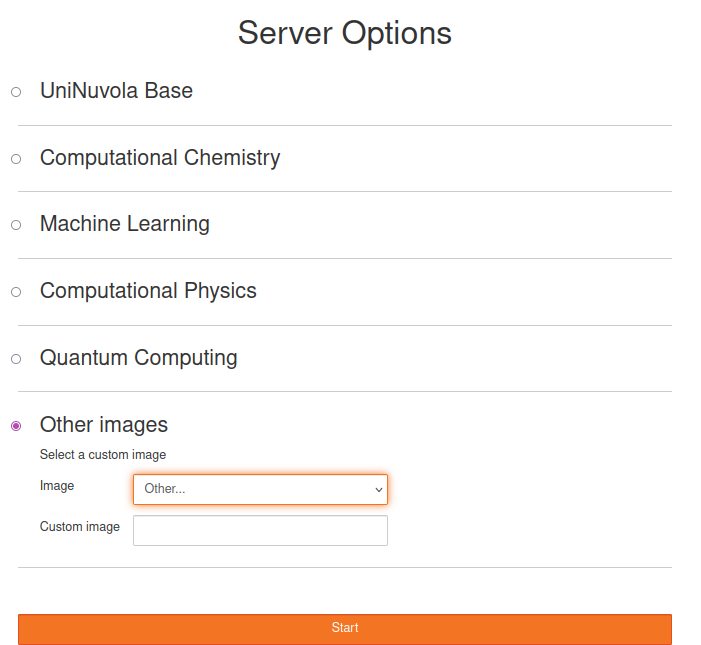
\includegraphics[width=0.75\textwidth]{figures/imageselecton.png}
    \caption{Jupyterhub's image selection page. }
    \label{image_selection}
\end{figure}


\section{Brief description of Jupyterhub}
JupyterHub provides a flexible, scalable, and secure environment for interactive computing. It is a multi-user platform designed for running Jupyter Notebook servers. As a user, you can access individual Jupyter Notebook instances to create and run notebooks, which support multiple programming languages, most commonly Python and R.\\ 

Depending on the future policies of \uninuvola, you will have access to specific computational resources (CPU,GPU,RAM...) allocated to your notebook instance. Your work and data are typically stored persistently, meaning that your files will be saved and available each time you log in.\\

Figure \ref{homepage} shows the homepage for the \uninuvola  ``Default''. The first line of shows all the available notebooks, in this case the classic Jupyter notebook and an Xpra terminal (see Section \ref{xpra}). The default offers a terminal, a general, a Python and Markdown text editors. \\
\begin{figure}[htbp]
    \centering
    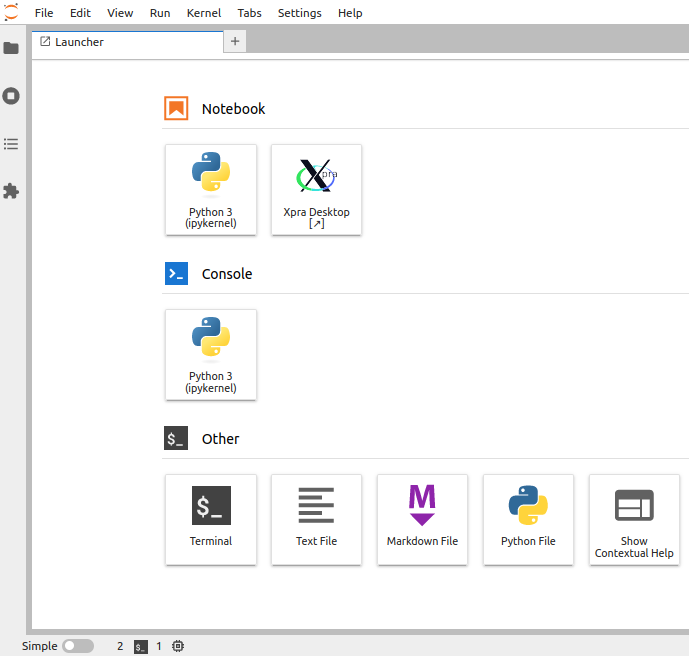
\includegraphics[width=0.75\textwidth]{figures/homepage.png}
    \caption{Homepage of your Jupyterhub home page. }
    \label{homepage}
\end{figure}


\subsection{Xpra}\label{xpra}

Xpra,\cite{Xpra} which stands for "X Persistent Remote Applications," is an innovative open-source tool designed for remote desktop and application forwarding. It allows users to run X11 programs on a remote server while displaying them locally, offering a seamless and flexible remote application experience.\\

With Xpra, you can operate graphical applications on a remote server as if they were running on your local machine, enabling the use of resource-intensive applications on powerful remote servers from a lightweight local client. Another significant advantage of Xpra is session persistence: it allows you to disconnect and later reconnect to your sessions without losing any work. Xpra employs advanced compression techniques and adapts to varying network conditions, ensuring smooth performance even over slower connections. It supports SSH encryption to secure communications between the client and server and can also be configured to use SSL/TLS for additional security. \\

Xpra also facilitates clipboard and audio forwarding, allowing seamless sharing of text or files between local and remote environments and enabling audio streaming from remote applications to your local machine. \\











%\section{Creation of the \textit{.bashrc} file}
%The \textit{.bashrc} file is a powerful tool to customise your Bash environment. It  is a script file %that Bash reads every time it starts a new interactive shell session. It's commonly used to configure %and customise the Bash environment for individual users.  \\ 

%During your first usage of the terminal in \uninuvola, or if you need to recreate your \textit{.bashrc} %file, run the conda initialisation for generating the \textit{.bashrc} file:


%\begin{lstlisting}[language=bash]
%$ bash
%jovyan@jupyter-mp890089$ /opt/conda/bin/conda init
%jovyan@jupyter-mp890089$ source .bashrc
%(base) jovyan@jupyter-mp890089$
%\end{lstlisting}

%This file is used by all the images inside \uninuvola.

